
\chapter{Important Concepts}
\label{chap:Concepts}
In this chapter, we present the most important building blocks on which this work is based. The goal is to give the necessary insights to allow a self-containing consumption of this thesis and place the work in a larger context. The three building blocks are the Transmission Control Protocol (TCP), the Multipath TCP (MPTCP) based on it and the new internet architecture SCION. These three concepts are summarized in the corresponding order in the following sections.

\section{Transmission Control Protocol (TCP)}
\label{sec:TCP}

This recap about the widely used transport protocol TCP is mainly inspired by the summary \cite{TCPSummary}.

The Transmission Control Protocol (TCP) is one of the main protocols in today's Internet. Its two main developers Vint Cerf and Bob Kahn started working on the protocol in 1974. The original specification was written in 1981; defined in the RFC document number 793 \cite{rfc793}.

TCP is a byte stream, connection-oriented and reliable transport protocol. In the OSI model, it is situated between the application layer above and the network layer below. TCP receives the data in a byte stream from the application. It is up to the protocol to partition this stream into so-called TCP segments in order to transmit the data in manageable pieces to the receiver. Before two endpoints can exchange data over TCP, they must first agree upon the willingness to communicate; hence connection-oriented. Similar to a call with a telephone, first a connection has to be established before the two parties can exchange information. We describe the procedure of a TCP connection establishment and termination later in this section. To ensure reliable data transfer TCP uses different mechanisms. A per-segment checksum enables the receiver to detect crudities in the transferred data. Everything that is received multiple times, is discarded by the receiving side. It is also the receiver that ensures that the received data is transferred to the application in the correct order. TCP also has a retransmission functionality that ensures delivery of the data in the case of data corruption or loss. The successful reception of data is confirmed by the receiver with a positive acknowledgment. If the sender does not receive such positive acknowledgments for a certain period of time, it will resend the data. 

\subsection*{TCP Segment}

TCP partitions the byte stream into TCP segments consisting of a header and a data part. Figure \ref{fig:TCPSegment} depicts a valid format of a TCP segment with its different fields. In the following, the fields most important for the understanding of the TCP are described in more detail. 

\begin{figure} [H]
	\begin{center}
		\def\svgwidth{1\textwidth}
		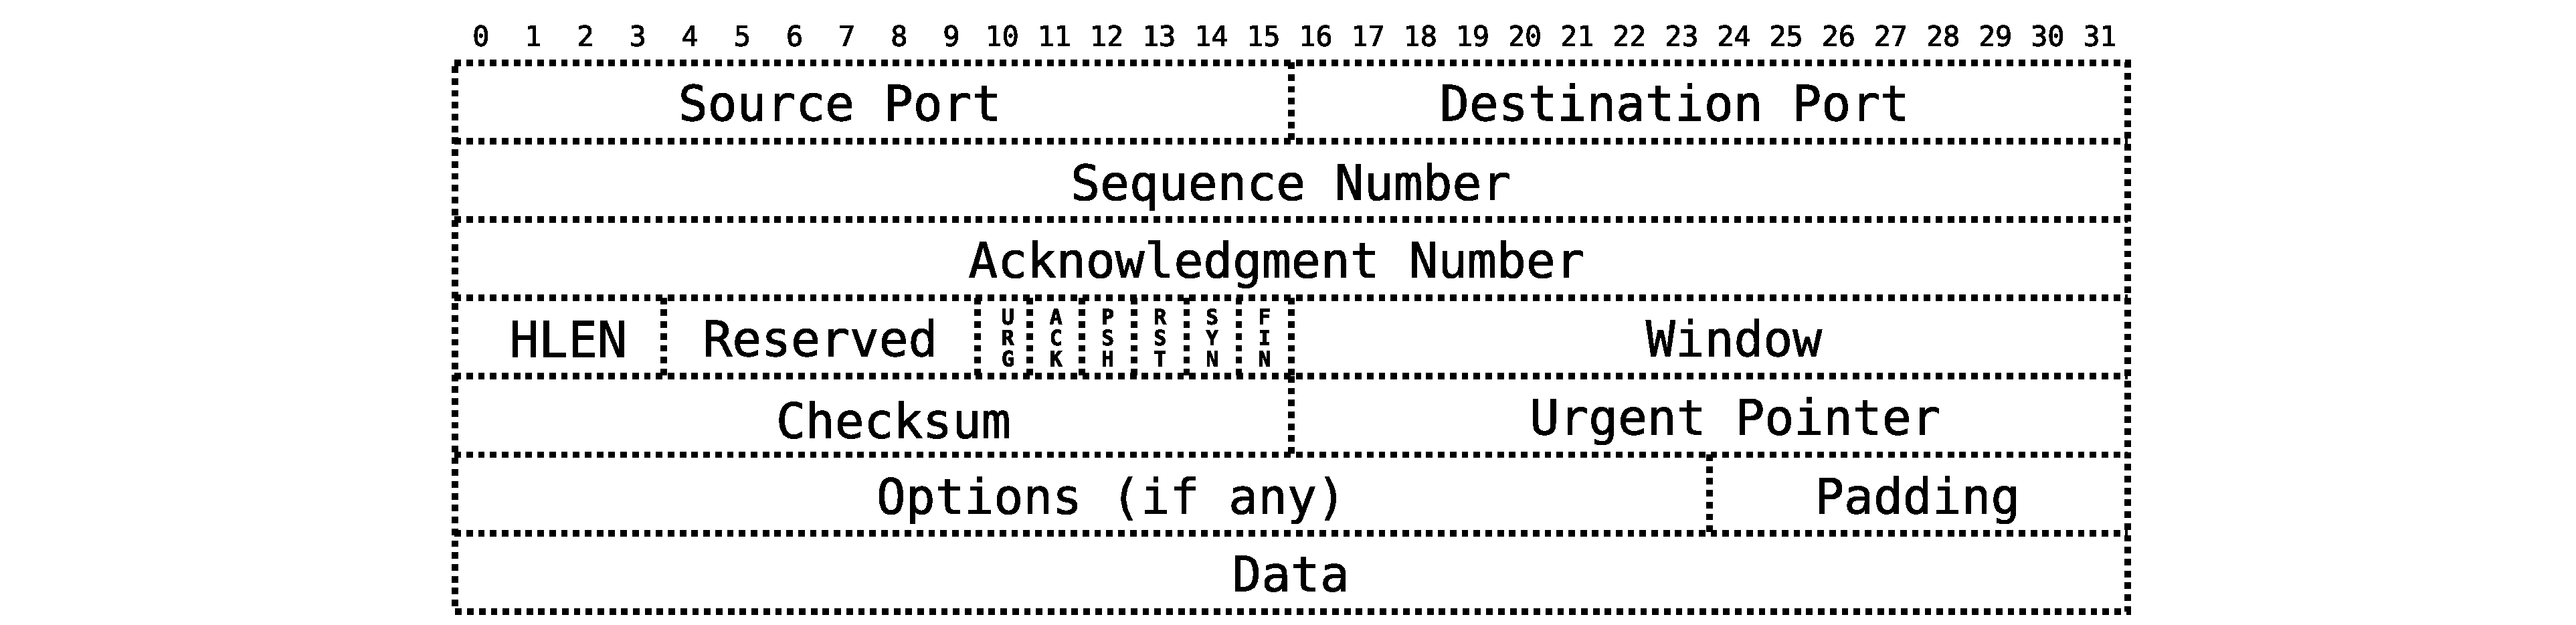
\includegraphics[scale=0.2]{../illustrations/importantConcepts/TCPSegment.pdf}  
		\caption[]{Illustration of a TCP segment.}
		\label{fig:TCPSegment}
	\end{center}
\end{figure}

{\small \textbf{Source Port:} 16-bit number tagging the application where the segment originated from within a sending endpoint. \smallskip\\
\textbf{Destination Port:} 16-bit number tagging the application where the segment is destined for on a receiving endpoint. \smallskip\\
\textbf{sequence number:} 32-bit number identifying the current position of the first data byte in the segment within the entire byte stream for the TCP connection. \smallskip\\
\textbf{Acknowledgment Number:} 32-bit number telling the receiver which data byte the sender is expecting next. It is always one greater than the most recently received data byte and only valid if the ACK control bit is set. \smallskip\\
\textbf{ACK (Control Bit):} If set, the acknowledgment number is valid. \smallskip\\
\textbf{Window:} 16-bit number used by TCP for flow control. It specifies the number of bytes the sender of this segment is currently willing to receive. \smallskip\\
\textbf{SYN (Control Bit):} Sender and receiver use this bit during the connection establishment to synchronize their sequence numbers.  \smallskip\\
\textbf{FIN (Control Bit):} This bit is part of the connection termination. It is set by the sender if its byte stream has reached the end. \smallskip\\
\textbf{Options:} Provides space for additional optional parameters that one may want to exchange between sender and receiver. 
}
 
Note that a single TCP connection is uniquely identified by a complete pair of IP addresses (source and destination) together with a complete pair of TCP ports (source and destination).

\subsection*{Connection Establishment, Data Transfer and Termination}

TCP is connection-oriented, meaning that there is a virtual connection between two endpoints exchanging data. Such a virtual connection runs through three stages: connection establishment, data transfer and connection termination.

\paragraph{Connection Establishment}

Two hosts, A and B, willing to communicate establish a connection by exchanging a predefined set of messages known as the Three-Way Handshake. Figure \ref{fig:TCPConnectionEstablishmentAndTermination} on the left side illustrates this sequence. 

\begin{figure}[H]
	\begin{center} 
		\def\svgwidth{1\textwidth}
		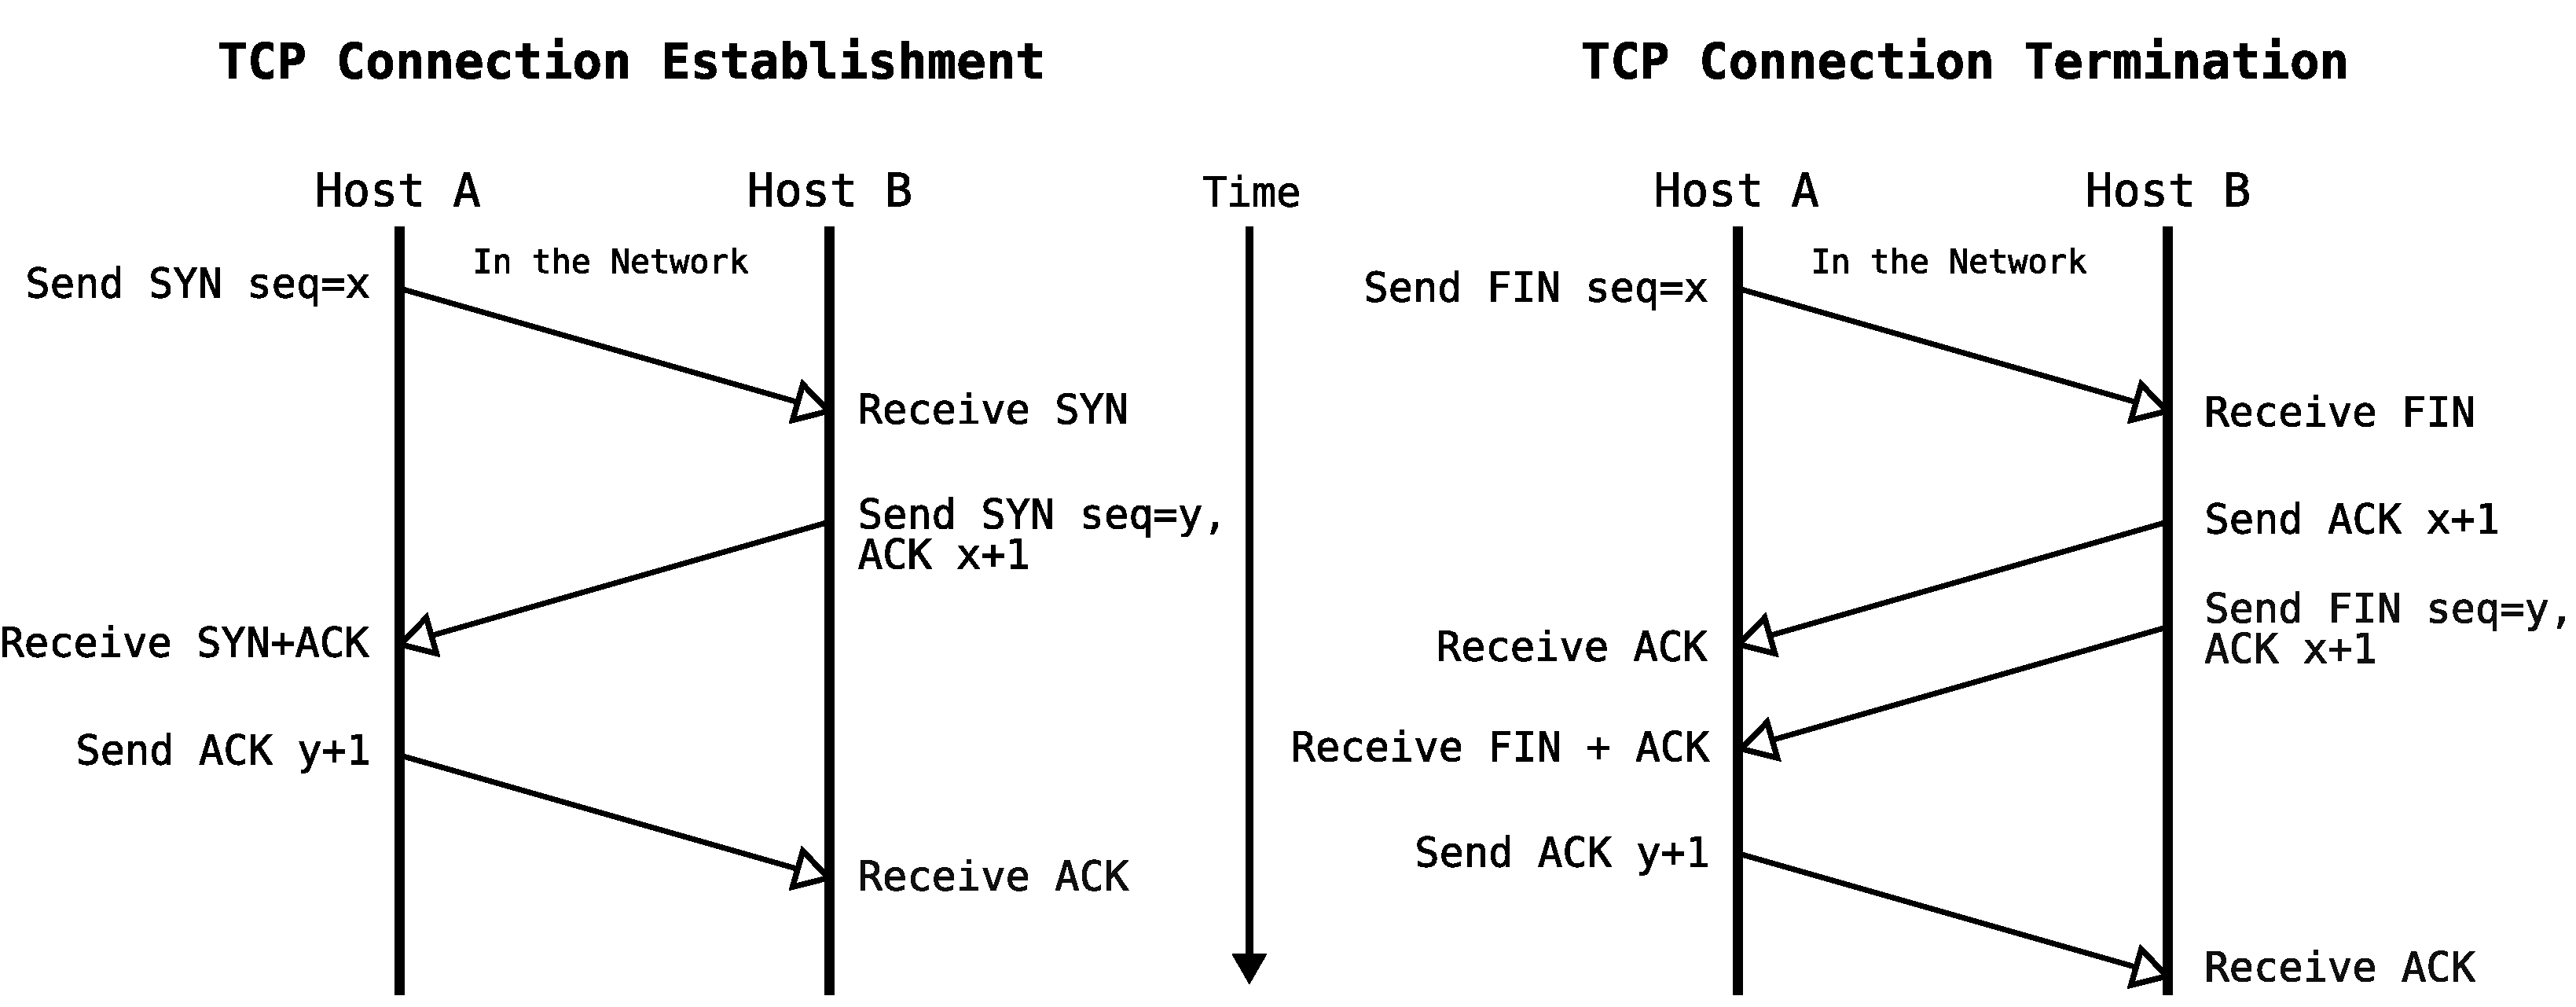
\includegraphics[scale=0.24]{../illustrations/importantConcepts/TCPHandshake.pdf} 
		\caption[]{Illustration of the TCP connection establishment (l.) and TCP connection termination (r.) messages exchange.}
		\label{fig:TCPConnectionEstablishmentAndTermination}
	\end{center}
\end{figure}

Host A as an initiator of the connection sends a segment containing an initial sequence number x and the SYN control bit set to Host B. \smallskip\\Host B processes the received segment and answers with a segment of its own. It contains an initial sequence number y and has the SYN control bit set. Furthermore Host B assigns x+1 to the acknowledgment number and sets the ACK control bit. This indicates that the next byte expecting from Host B should contain data starting with sequence number x+1. \smallskip\\ Host A finishes the connection establishment phase upon reception of Host B's SYN+ACK. It sends a last acknowledgment to Host B, indicating that the next expected byte should start with sequence number y+1.

\paragraph{Data Transfer}

Once the Three-Way Handshake is completed, the two hosts can exchange data with each other. Important functionalities of the data transfer are flow control and congestion control. These concepts are discussed later, first the focus lies on some key ideas.

In a basic TCP implementation, segments are put into the network by the sender as long as there is data available and as long as the window announced by the receiver is not exceeded. The receiver consumes the segments and acknowledges them by sending back positive acknowledgments together with its current position in the byte stream. The announcement of the current window size is also included in these messages sent back. If data gets lost or duplicated, a hole may exist in the byte stream. The receiver continues to acknowledge the most current contiguous position in the byte stream accepted so far.

The sender must halt transmission in the case where data ready to be sent will exceed the receivers advertised window size. Upon reception of further positive acknowledgments announcing a window size greater than zero, the sender can continue delivering the data.

If there is no data to send, TCP waits patiently until either there is some again or the other end of the connection sends data to receive.  

\paragraph{Connection Termination}

A TCP connection is completely terminated by the exchange of four segments as depicted on the right side of Figure \ref{fig:TCPConnectionEstablishmentAndTermination}. Since the protocol is full-duplex, both ends must be torn down independently. To initiate this process the FIN control bits are used. 

As soon as the application running on Host A wants to close the connection, a FIN segment is sent from Host A to Host B. Upon reception of this segment, Host B acknowledges it and notifies its destination application about the termination request. As soon as this application shuts down the connection as well, Host B sends out a FIN segment which is finally acknowledged by Host A.

\subsection*{Flow Control}

Flow control is an important part of the data transfer in TCP. Its purpose is to properly match the transmission rate of the sender to the one of the receiver and the network. For performance reasons, one is interested in a transmission rate that is high enough without overwhelming the receiver or the network. TCP uses the window field to adjust the rate of flow between TCP endpoints. This concept is called sliding window. In every segment, the receiver specifies with the window field how much data it is willing to buffer. The sender can only send up to that amount of data before it has to wait for further acknowledgments and window updates from the receiver. 

\subsection*{Congestion Control}

Another major part of the data transfer in TCP is congestion control. However, this term is misleading, since it rather should be called congestion avoidance. TCP itself cannot control the congestion, it rather tries to avoid congestion using different mechanisms, which are briefly discussed in the following. 

\paragraph{Slow Start}

Slow start is a mechanism used by the sender to control the sending rate. Hereby, the rate of acknowledgments returned by the receiver controls the rate at which the sender can transmit data. At the very beginning of a TCP connection, the congestion window is initialized to one. With every positive acknowledgment received, the congestion window is increased by one. The sender can send the minimum of this congestion window and the advertised window of the receiver, denoted as transmission window. Unlike the name suggests, slow start is by no means slow. In a congestion-free network with good response time, the congestion window doubles for every round-trip-time. The increase of the congestion window will continue until the maximum transmission window is reached or until congestion finally occurs.

\paragraph{Congestion Avoidance}

The congestion avoidance algorithm has two mechanisms to detect network congestion. If the blockage is indicated through the reception of duplicate acknowledgments, the transmission window is halved and the fast retransmit and fast recovery mechanism take over. If the congestion was indicated through a timeout of the retransmission timer, the sender is put back into slow start mode, i.e. the transmission window is set to one. After running into congestion, the congestion window is again increased using slow start. However, it is only used up to the halfway point where congestion originally occurred. After reaching this point, the congestion window is just increased by one for all segments in the transmission window that are acknowledged. The linear growth from this point onward makes sure that TCP increases its transmission rate more slowly towards the previous congestion point.  

\paragraph{Fast Retransmit}

If the sender receives an acknowledgment multiple times, it is not clear if it is because a segment was lost or simply because a segment was delayed and received out of order at the receiver. If the latter is the case, it should not take too long until the latest expected acknowledgment arrives. Typically, for simple out of order condition, not more than one or two duplicated acknowledgments should be received. More duplicates are a strong indication that a segment was lost. Upon reception of three duplicated acknowledgments, the sender does not wait until the retransmission timer expires but resends the segment immediately and enters Fast Recovery.

\paragraph{Fast Recovery}

Duplicate acknowledgments can only be generated when a segment is received at the receiver. Therefore, as long as the sender receives acknowledgments it knows that there is data flow through the network. The loss of a segment was probably just a rare event, instead of reducing the flow drastically by using slow start again the sender just enters congestion avoidance without decreasing the size of the congestion window too much. This behavior allows for higher throughput in cases of only moderate congestion.

\subsection*{Conclusion}

TCP is a rather complex protocol that handles an enormous amount of functionality in today's Internet. The presented discussion gives only a small insight into the scope of TCP. However, it provides the necessary insights to understand the extensions to TCP, namely Multipath TCP, discussed in the next section.

\section{Multipath TCP (MPTCP)}
\label{sec:MPTCP}

In this section, we introduce Multipath TCP. The presented summary is based on \cite{Barre2011, Raiciu2012, Wischik2011} and the RFC document number 6824 \cite{rfc6824}.

\subsection*{Basics}

In times where most hosts are equipped with multiple physical interfaces, a protocol that binds each connection to a single interface does not exhaust the potential of the infrastructure. TCP is not capable of using the multiple paths to the Internet available for an increase in connection redundancy and performance. Multipath TCP, as an evolution of TCP, is an attempt to utilize the multiple paths available to gain robustness and performance advantages.

Multipath TCP allows an unmodified application to start what it believes a regular TCP connection using the well-known API for TCP. If both endpoints support the use of MPTCP, multiple flows are established under the hood. The data is shared among these flows, where most data is sent out on the least congested path. If the use of MPTCP is not supported a regular TCP connection is established instead. Multipath TCP works in all scenarios where TCP currently works. By using an appropriate congestion control MPTCP furthermore ensures that other, regular TCP connections present in the network are not disadvantaged. 

\subsection*{Connection Setup}

MPTCP uses the TCP Three-Way Handshake to set up the initial connection, i.e. the main-flow. The sender includes the MP\_CAPABLE option in the SYN, which is also included in the returning SYN+ACK when the server is ready to use MPTCP. The sender concludes the Multipath TCP connection setup by including the MP\_CAPABLE option in the third packet of the handshake as well. The connecting entities fall back to regular TCP if not all segments being exchanged as part of the Three-Way Handshake contain the respective option. The MP\_CAPABLE option itself contains a 64-bit key generated by the sender and the receiver, later used to verify the authenticity of additional flows. The sequence of segments exchanged for an MPTCP connection establishment between two Host A and B is illustrated in Figure \ref{fig:MTCPConnectionEstablishment}.

\begin{figure}[H]
	\begin{center} 
		\def\svgwidth{1\textwidth}
		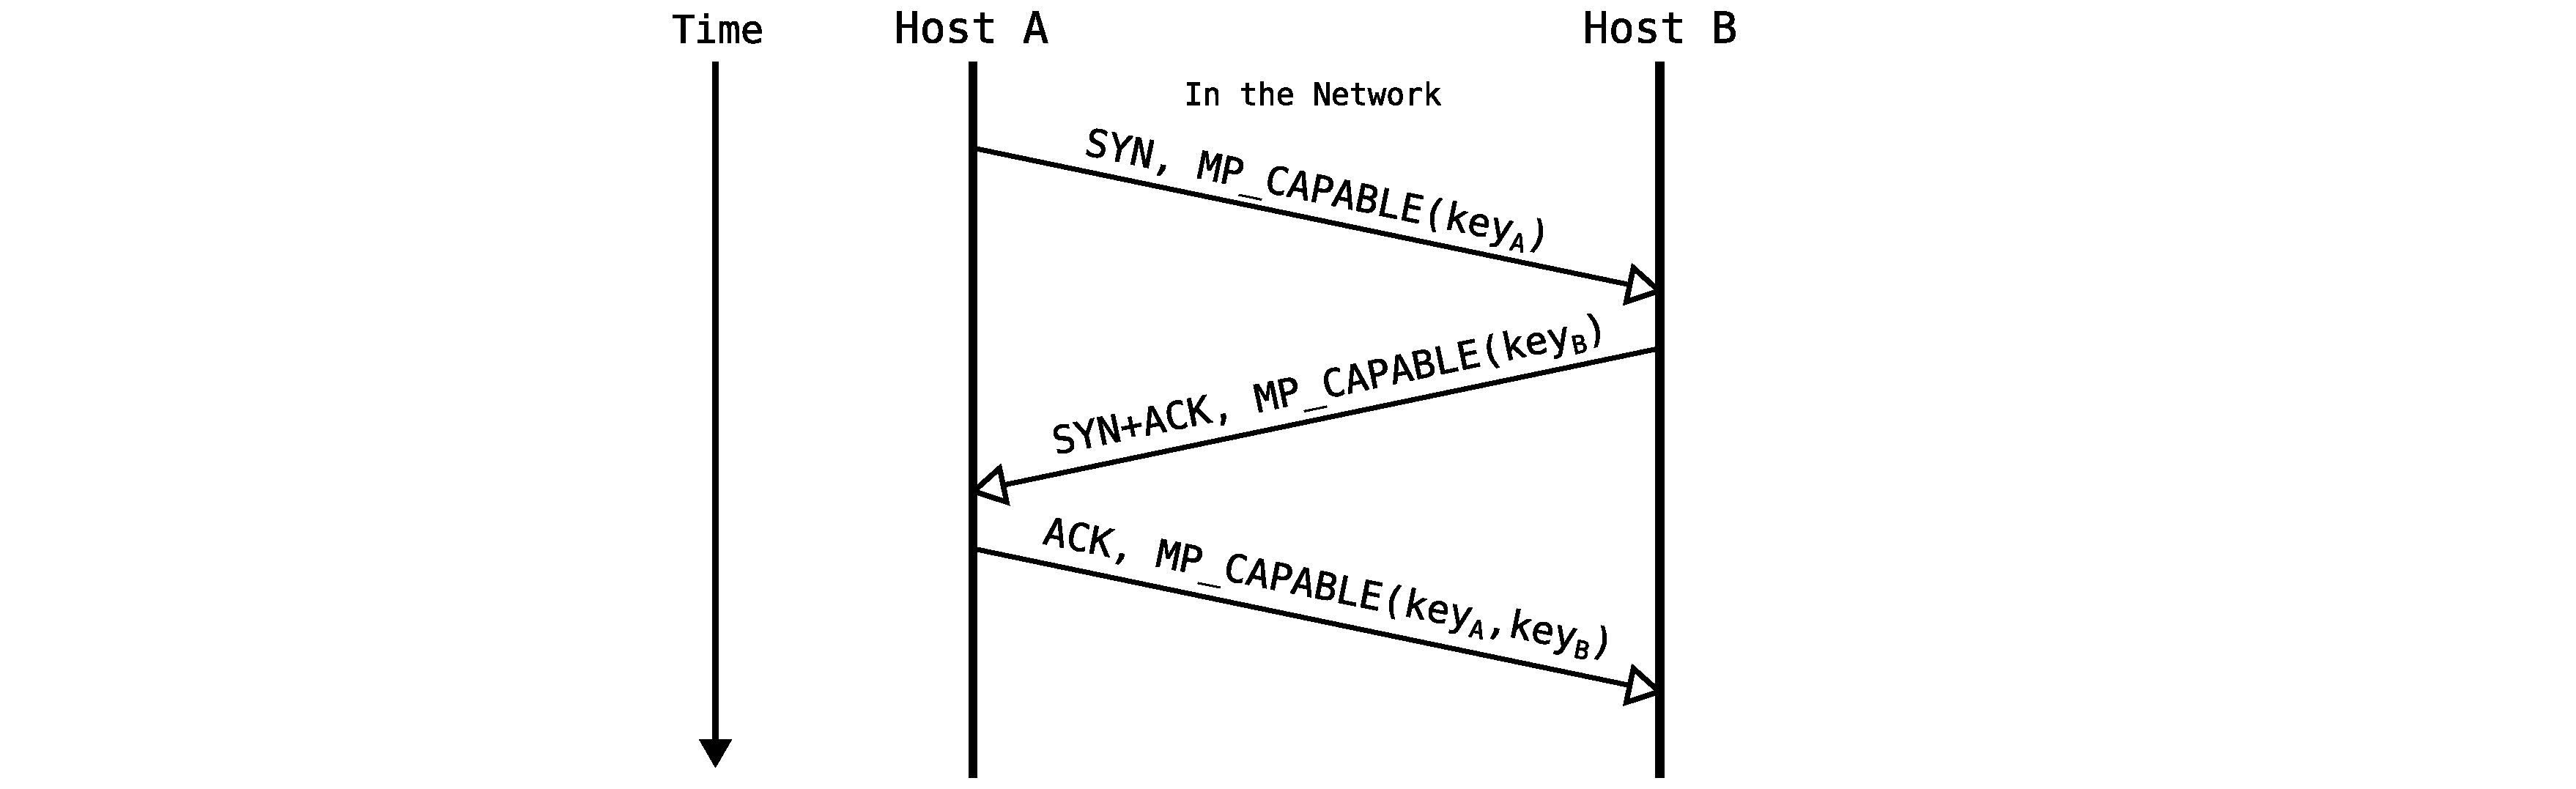
\includegraphics[scale=0.24]{../illustrations/importantConcepts/MPTCPHandshake.pdf} 
		\caption[]{Illustration of the sequence of segments exchanged for the MPTCP connection setup. The MP\_CAPABLE option has to be included in all messages exchanged for the establishment to succeed.}
		\label{fig:MTCPConnectionEstablishment}
	\end{center}
\end{figure}

\subsection*{Addition of Sub-flows}

Once a connection, i.e. the main-flow, has been established, further flows, so-called sub-flows, can be added. For this, MPTCP again performs a regular TCP Three-Way Handshake using addresses or ports of additionally available interfaces. To add the sub-flow, the MP\_JOIN option has to be included in any segment part of the handshake. This option holds the message authentication code (MAC) of the keys exchanged in the previously described initial connection setup. This measure makes it difficult for malicious third parties to hijack an existing connection. Furthermore, the option includes a connection identifier, derived as a hash from the receiver's key, used to match new sub-flows with an existing connections main-flow. 

\subsection*{Data Transfer}

Data exchanged between client and server can be sent over any flow part of a Multipath TCP connection. To remain a reliable protocol, MPTCP must retransmit data over a different flow if a certain flow fails. This is achieved by making use of two different principles discussed in the following and illustrated in Figure \ref{fig:MPTCPDataTransfer}.

\paragraph{Flow and Data Sequence Number}

In Multipath TCP every flow is equivalent to a regular TCP connection using its own 32-bit sequence number space. With this flow sequence number, the current position within the entire byte stream transferred over a certain flow is identified. Additionally, MPTCP maintains a 64-bit data sequence numbering space, which is used by the DSS\_MAP and the DSS\_ACK option. The DSS\_MAP contains a mapping between the flow sequence number and the data sequence number. It is used by the receiver for correctly ordering the byte stream, possibly received disordered over the different flows, for the application.

\paragraph{Two different Acknowledgment Levels}

The acknowledgment of received data happens on two different levels. The regular TCP acknowledgment Number is used to confirm the reception of data on a flow connection level. Standard retransmission mechanisms, as discussed earlier, are used to recover from a segment loss indicated through the reception of multiple acknowledgments confirming the same flow sequence number. With the additional DSS\_ACK returned by the receiver as part of the ACK's, cumulative acknowledgments at a data sequence level are available. These allow MPTCP to detect the failure of a flow and to initiate the retransmission of lost data over a different flow.

\begin{figure}
	\begin{center}
		\def\svgwidth{1\textwidth}
		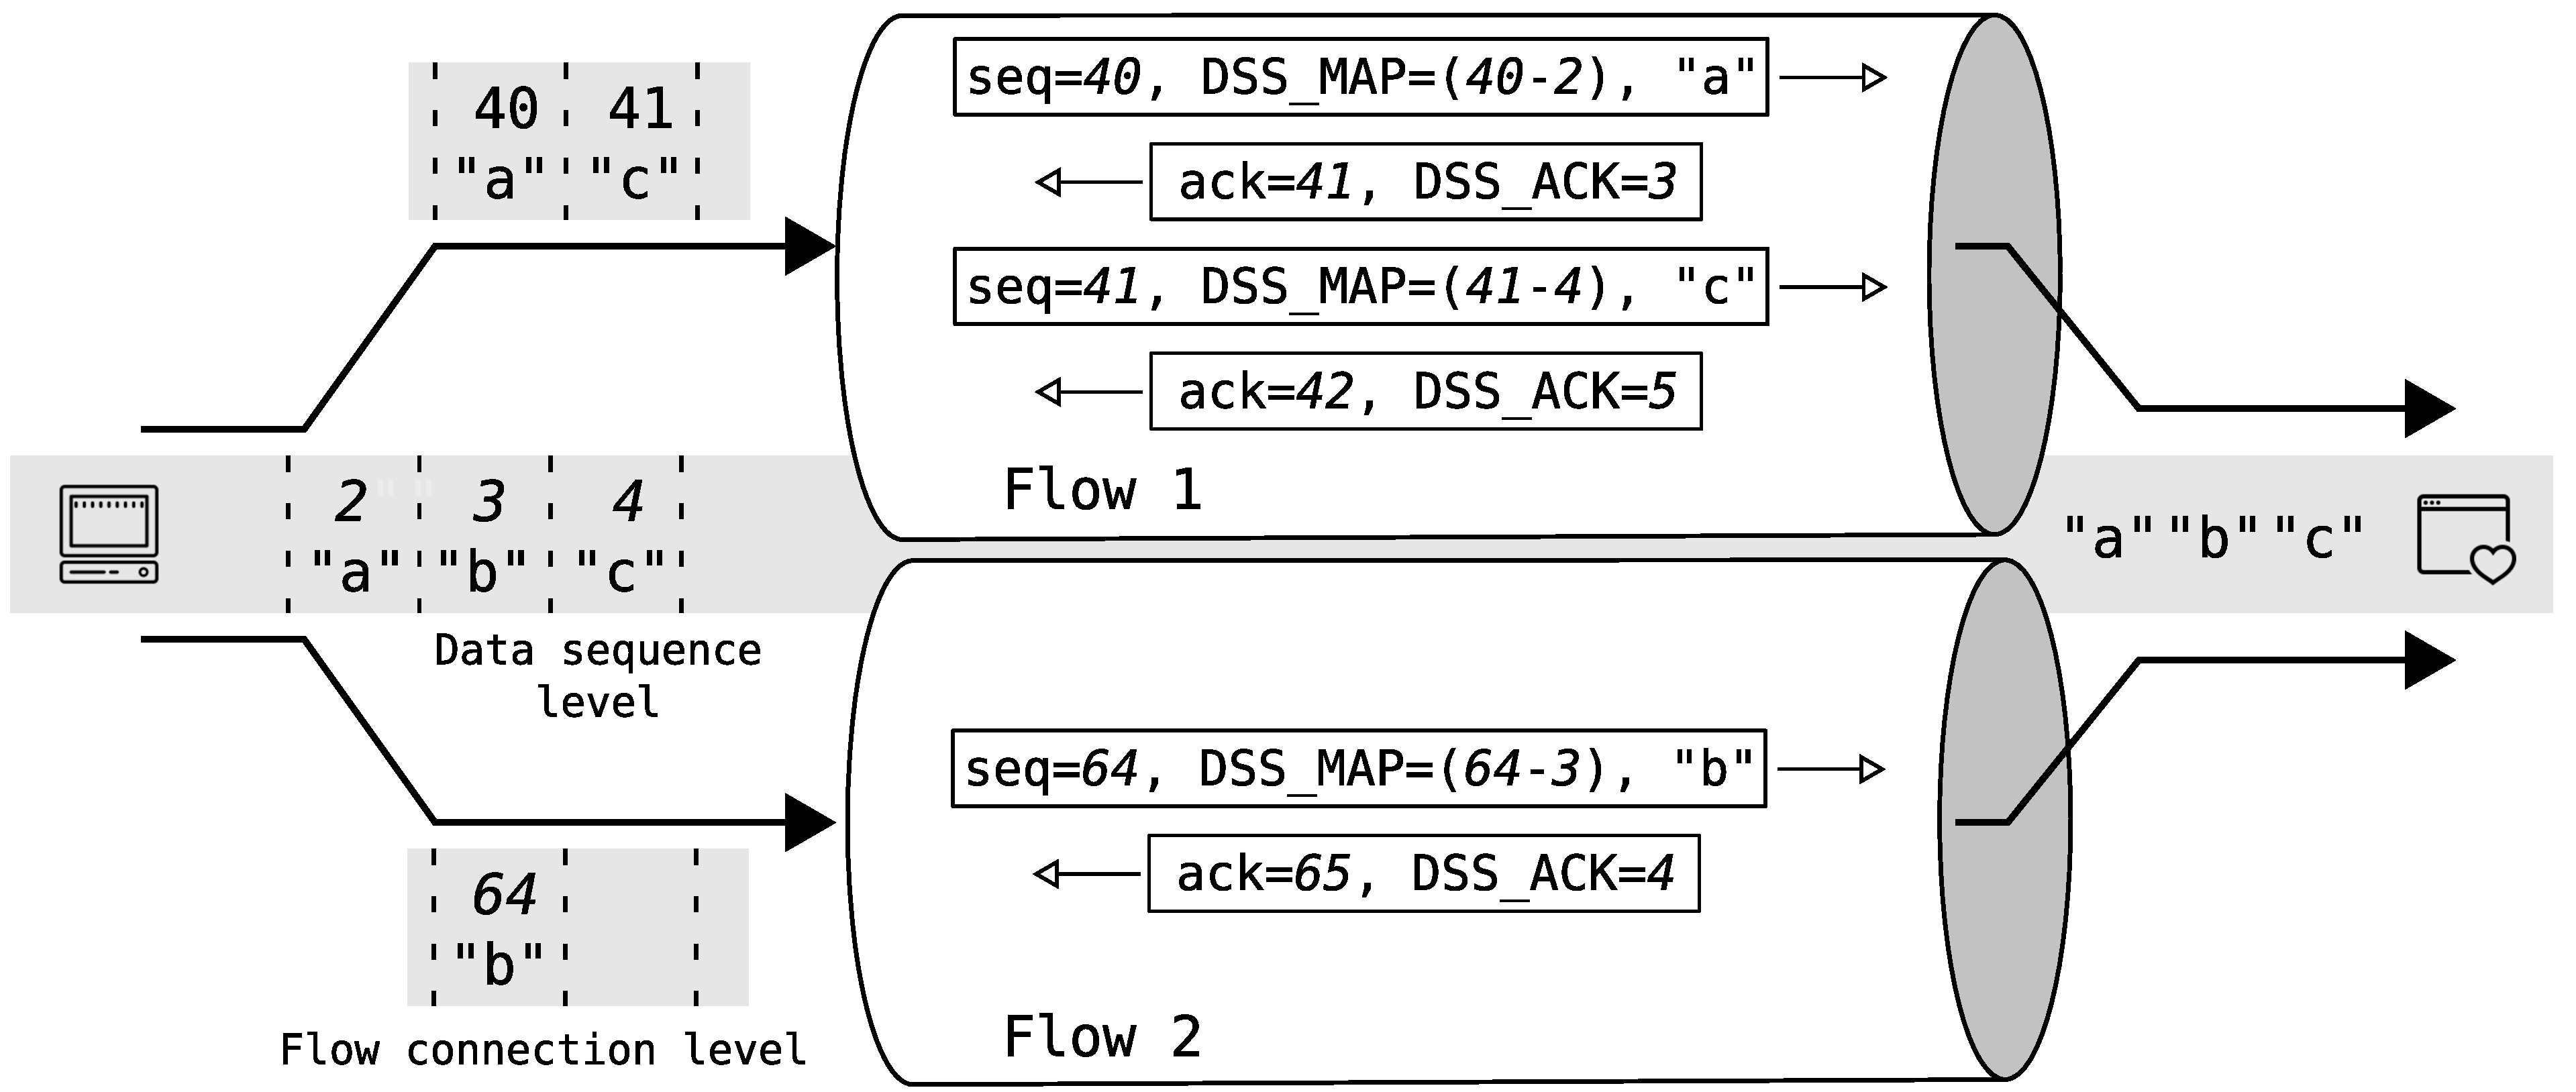
\includegraphics[scale=0.2]{../illustrations/importantConcepts/MPTCPDataTransfer.pdf}  
		\caption[]{Illustration of data transfer in MPTCP with two flows. The regular TCP sequence numbers are used to acknowledge data reception and trigger mechanisms for re-transmission on a flow connection level. With the additionally introduced DSS\_ACK's on a data sequence level, MPTCP is able to detect dying flows and can maintain the ordering of exchange data.}
		\label{fig:MPTCPDataTransfer}
	\end{center}
\end{figure}

\subsection*{Congestion Control}

One way to implement congestion control in MPTCP is to use conventional mechanisms on a flow connection level. This means that each TCP flow maintains its congestion window without affecting or being affected by other flows and their window. Possible congestion control could be any suitable for TCP, like the default AIMD approach \cite{rfc5681} mentioned in the previous section or derivatives like CUBIC \cite{rfc8312}. But with independent congestion windows for each flow, other users in the network are disadvantaged. Imagine that several flows of an MPTCP connection and a single external TCP connection share the same link. In this case, the MPTCP may use more bandwidth than it is entitled to.  This is possible because each flow is treated as a single, independent TCP connection. To eliminate this injustice MPTCP uses a congestion algorithm which makes the windows of the individual flows dependent on each other. One possible implementation hereby is the Linked Increase Algorithm (lia) \cite{rfc6356}, initially proposed by the community.  In the meantime, further developments, for example the Opportunistic Linked Increase Algorithm (olia) \cite{khalili-mptcp-congestion-control-05}  or the Balanced Linked Adaptation Congestion Control Algorithm (balia) \cite{walid-mptcp-congestion-control-04} are available.

\subsection*{Conclusion}

The benefits of MPTCP as an extension are promising, as already mentioned in Chapter \ref{chap:RelatedWork}, especially in the area of smartphone usage.  With this summary, we have by no means covered all facets of Multipath TCP. But it does provide a basis for understanding this work and how we try to benefit from the protocol as well. An overview of the current development around MPTCP can be found here \cite{MPTCPWebMain}.

\section{SCION}
\label{sec:SCION}

In the upcoming summary, we introduce the fundamental concepts of SCION. It is based on the SCION book \cite{SCIONBook} and a selection of videos \cite{SCIONWebVideos}. More information and the latest news about the development of SCION can be found on the official web site \cite{SCIONWebMain}.

\subsection*{Shortcomings of today's Internet}

We start by mentioning some of the Internet's shortcomings, more precisely the shortcomings of two important building blocks of it. Today's Internet is of great importance for the economy, politics and society worldwide. Despite this importance, the global infrastructure does not meet the requirements in terms of security and availability to any degree. The core of the Internet is based on a few protocols developed almost 30 years ago. The Internet Protocol (IP) and the Border Gateway Protocol (BGP) control most system-relevant functions, but have undergone only minimal development since their deployment and suffer from several shortcomings.

\paragraph{Internet Protocol (IP) and its Shortcomings}

IP handles the transport of packets between end-users along a single path through the Internet. It routes them from a starting point to a destination, the endpoints have no influence on or knowledge of the path the packets take. All units involved in the routing determine the next hop based only on the destination address and a routing table. For IP, one can note the following shortcomings: The protocol does not sufficiently separate the functionality of routing and forwarding, sudden updates of routing tables can adversely affect a path, e.g. change its direction or even break it. Furthermore, the protocol does not offer the end-user with the possibility to control or check the path his data takes through the Internet. This functionality would be desirable in many situations, e.g. allowing a sender to avoid sending its data through malicious nodes. Furthermore, the IP protocol is based on the use of routing tables. The high-performance lookup of next-hop destinations is energy-intensive and the routing tables can be maliciously exhausted.

\paragraph{Border Gateway Protocol (BGP) and its Shortcomings}

BGP is responsible for the exchange of routing information between independently operating autonomous systems, denoted as ASes, like Internet service providers (ISPs). These providers use BGP update messages to announce the IP prefixes which are reachable through their subnet. Each ISP can decide based on its criteria, which announcements it wants to share further and which routes it wants to use. This traffic engineering is mainly driven by economically influenced policies. BGP also suffers from some shortcomings. It may take a considerable amount of time for the routing infrastructure to return to a stable state after new announcements have been made. Route changes directly affect forwarding and can lead to failures and interruptions of the data exchange. Furthermore, notifications affect all BGP entities that are present in the network. There is no hierarchy or isolation between individual areas. A single faulty BGP entity can severely disrupt the entire global routing infrastructure. Finally, BGP only allows one to select a single path for the routing between different autonomous systems. 

\subsection*{SCION - Scalability, Control and Isolation on Next-generation Networks}

Intending to remedy the above-mentioned shortcomings and create a better, safer internet, the development of SCION started with the publication of the first paper \cite{SCIONPaper} in 2011. SCION, an acronym for Scalability, Control and Isolation on Next-generation networks, shall become a secure network architecture that provides high availability regardless of the presence of malicious actors and offers efficient point-to-point packet delivery. In the ensuing section, we then give an introduction to the correspondingly implemented SCION architecture. Its implementation and design are guided by the following objectives.

{\small \textbf{High availability:} The functionality of the network is guaranteed even in the presence of a malicious party as long as at least one benign path exists between communicating endpoints. \smallskip\\
	\textbf{Path transparency:} Endpoints have control over and insight into the path their data takes through the network. \smallskip\\
	\textbf{Plane separation:} There is a strict separation of control plane and data plane which ensures that their functionality is not influenced by each other. \smallskip\\
	\textbf{Multipath support:} The architecture allows an endpoint to send data to its destination along multiple paths. \smallskip\\
	\textbf{Router state avoidance:} Routing works without the routers having to store a state.
}

\subsection*{The SCION Architecture}

The SCION architecture combines autonomous systems (ASes) into so-called isolation domains (ISD). Each ISD is managed by a subset of ASes, which form the ISD core and are denoted as core ASes. These core ASes agree on a policy, a trust root configuration (TRC), which applies inside their ISD and is used to validate bindings between names and public keys or addresses. Mapping to the real world, an isolation domain can for example represent a single state or the union of several states with the same legal understanding. Figure \ref{fig:SCIONArchitectureISDs} depicts a possible grouping of ASes into different ISDs connected by respective links.

\begin{figure}
	\begin{center}
		\def\svgwidth{1\textwidth}
		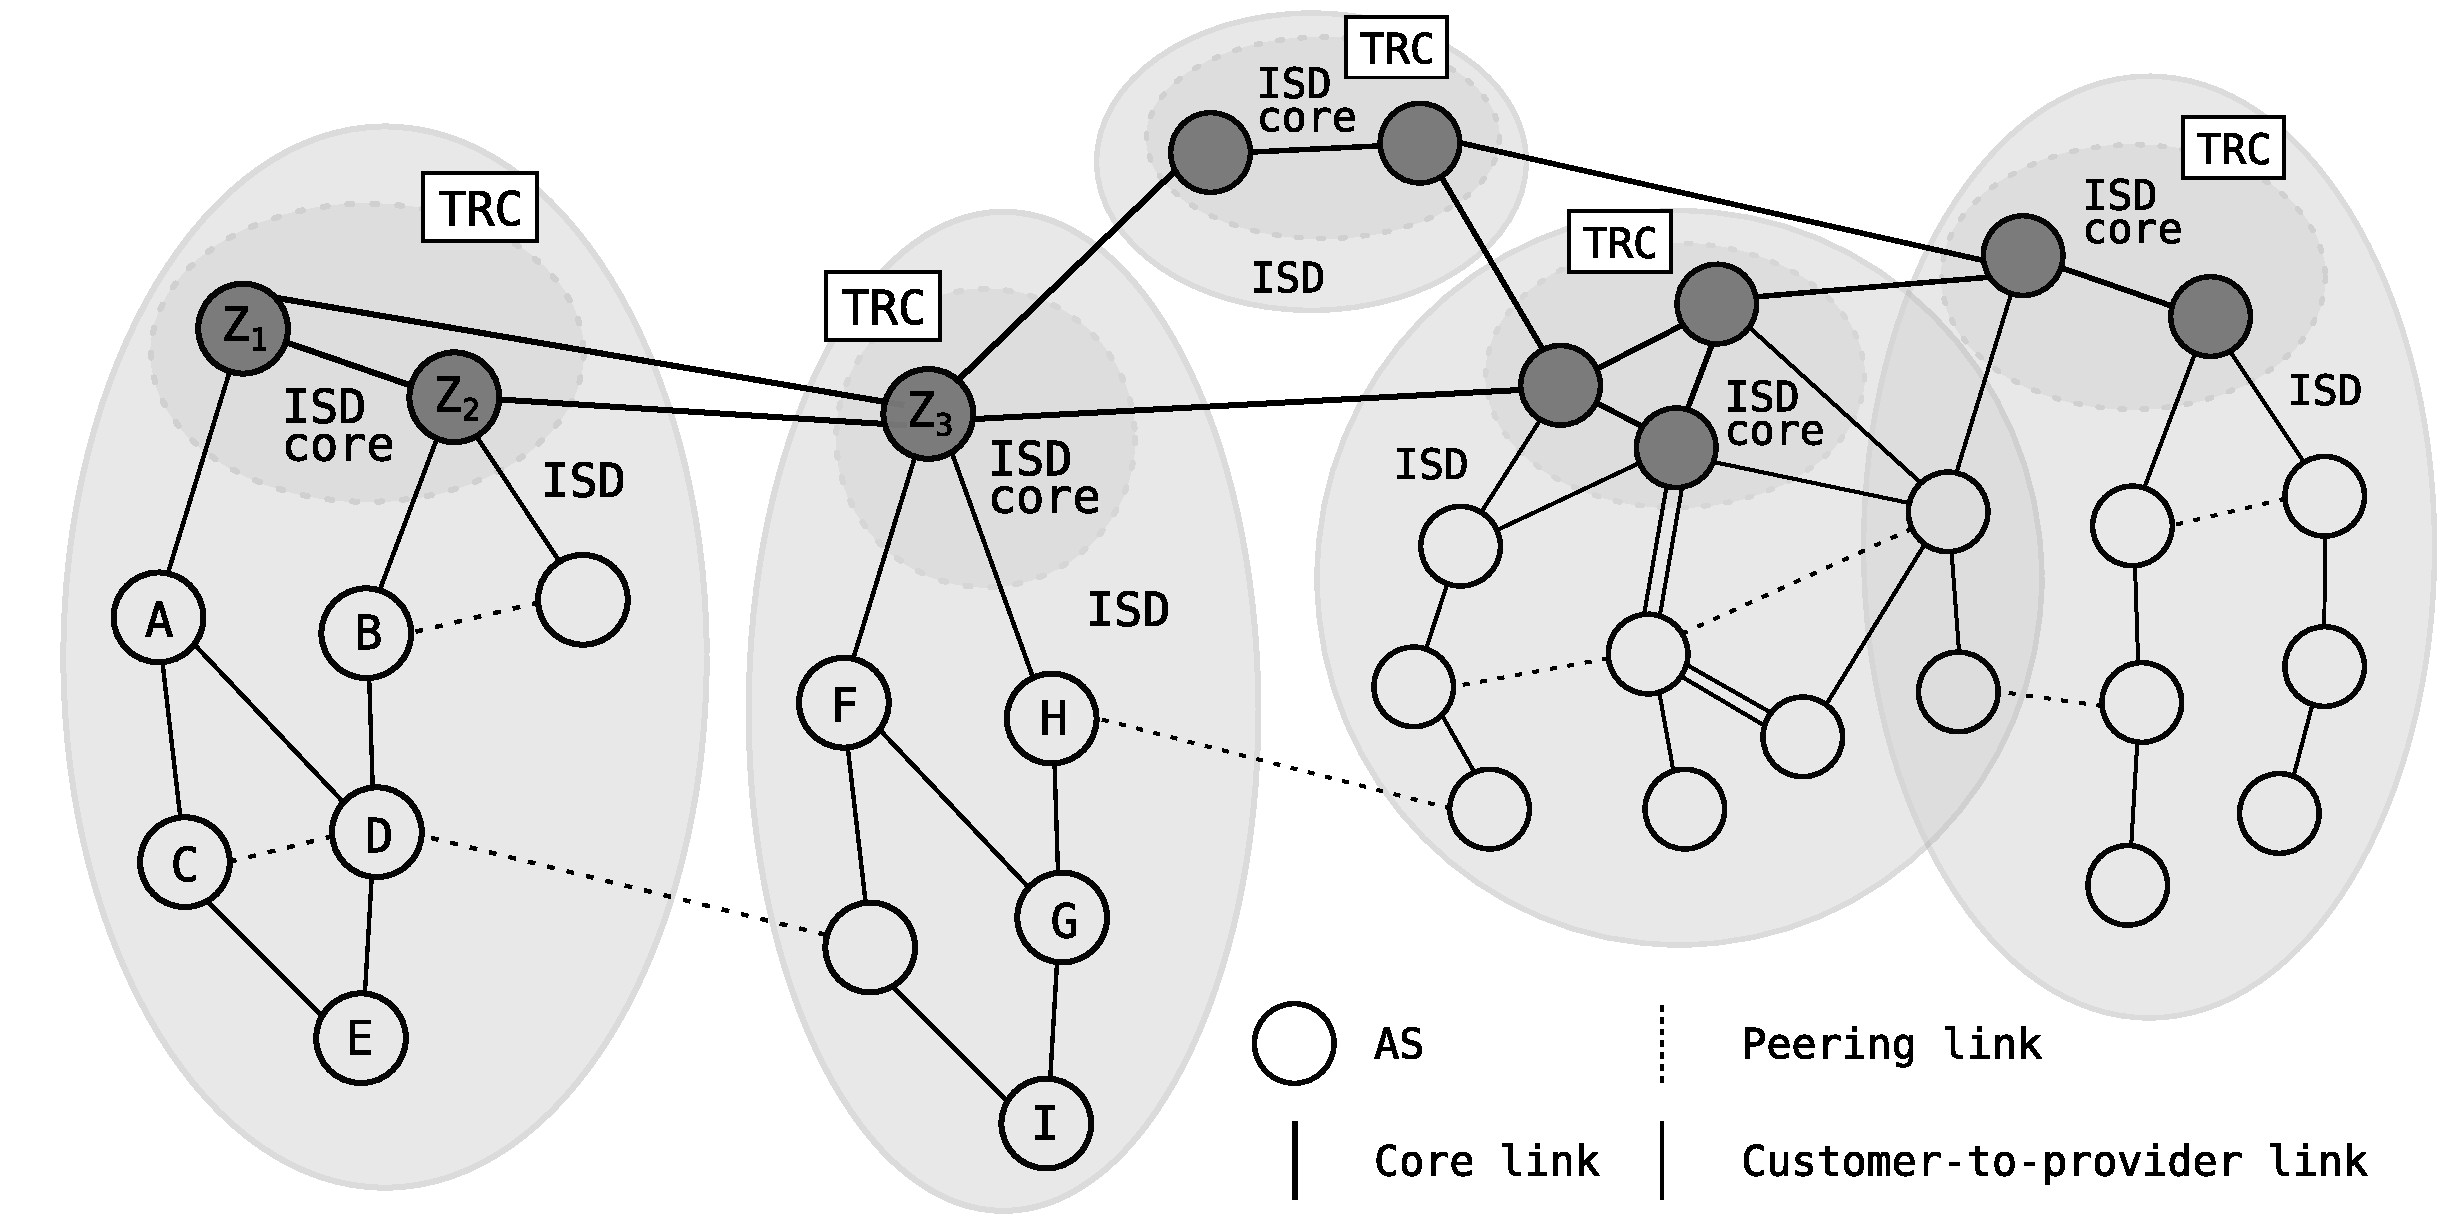
\includegraphics[scale=0.24]{../illustrations/importantConcepts/SCIONISDsAndASes.pdf} 
		\caption[]{Illustration of multiple ISDs with their ASes connected through different types of links. Core ASes via core links and ASes not belonging to the core via customer-to-provider or peering links. This drawing is inspired by the one shown in the SCION book \cite{SCIONBook} on page 18.}
		\label{fig:SCIONArchitectureISDs}
	\end{center}
\end{figure}

To enable an exchange between two endpoints, one or more paths through the network must be defined along where the data is sent. Every single step which is necessary to create such forwarding paths can be assigned to one of two planes. The control plane is responsible for discovering the paths and making them available to the end hosts, whereas the data plane is responsible for forwarding the data along the corresponding paths. This strict separation of routing (control plane) and forwarding (data plane) is one of the key features of SCION. The individual steps of creating a forwarding path are summarized below and illustrated in Figure \ref{fig:SCIONCreationForwardingPath}. The heading of the individual parts indicates their assignment to the corresponding plane.

\paragraph{Path Exploration (Control Plane)}

The first step in creating a forwarding path is path exploration, called beaconing in SCION terminology. The core ASes regularly send path-segment construction beacons (PCBs) to all its neighbors. Upon reception, an AS adds its own information and forwards the PCBs further to its neighbors. This results in a sequence of ASes representing a path through the SCION network. 

\paragraph{Path Registration (Control Plane)}

An AS typically receives several PCB's which describe path segments to different core ASes. It is up to each AS to decide which of the these it wishes to use. In the path registration, an AS registers the paths via which it wishes to be reached. For this purpose, the corresponding paths are registered at the path servers of the ISD, i.e. they are announced and thus available for the formation of forwarding paths. 

\paragraph{Path Lookup (Control Plane)}

If a source host wants to create a connection to a target host, it carries out a path lookup. From the path servers in the network, it receives path segments that can then be combined, as part of the data plane functionality,  into a forwarding path in a final step. 

\paragraph{Path Combination (Data Plane)}

After a host has received individual path segments in the course of the path lookup, it can now combine these into a path to the destination. Depending on where the destination is located, up to three path segments must be combined. If the destination AS is on the path from source AS to its core AS, then one segment is sufficient. If source and destination share only one core AS within the ISD, two segments are necessary, namely one from the source AS to the core AS and one from the core AS to the destination AS. Three path segments are necessary if source and destination are not located in the same ISD. In addition to the path segments connecting the ASes to their core, a segment between the two core ASes is necessary.

\begin{figure}
	\begin{center}
		\def\svgwidth{1\textwidth}
		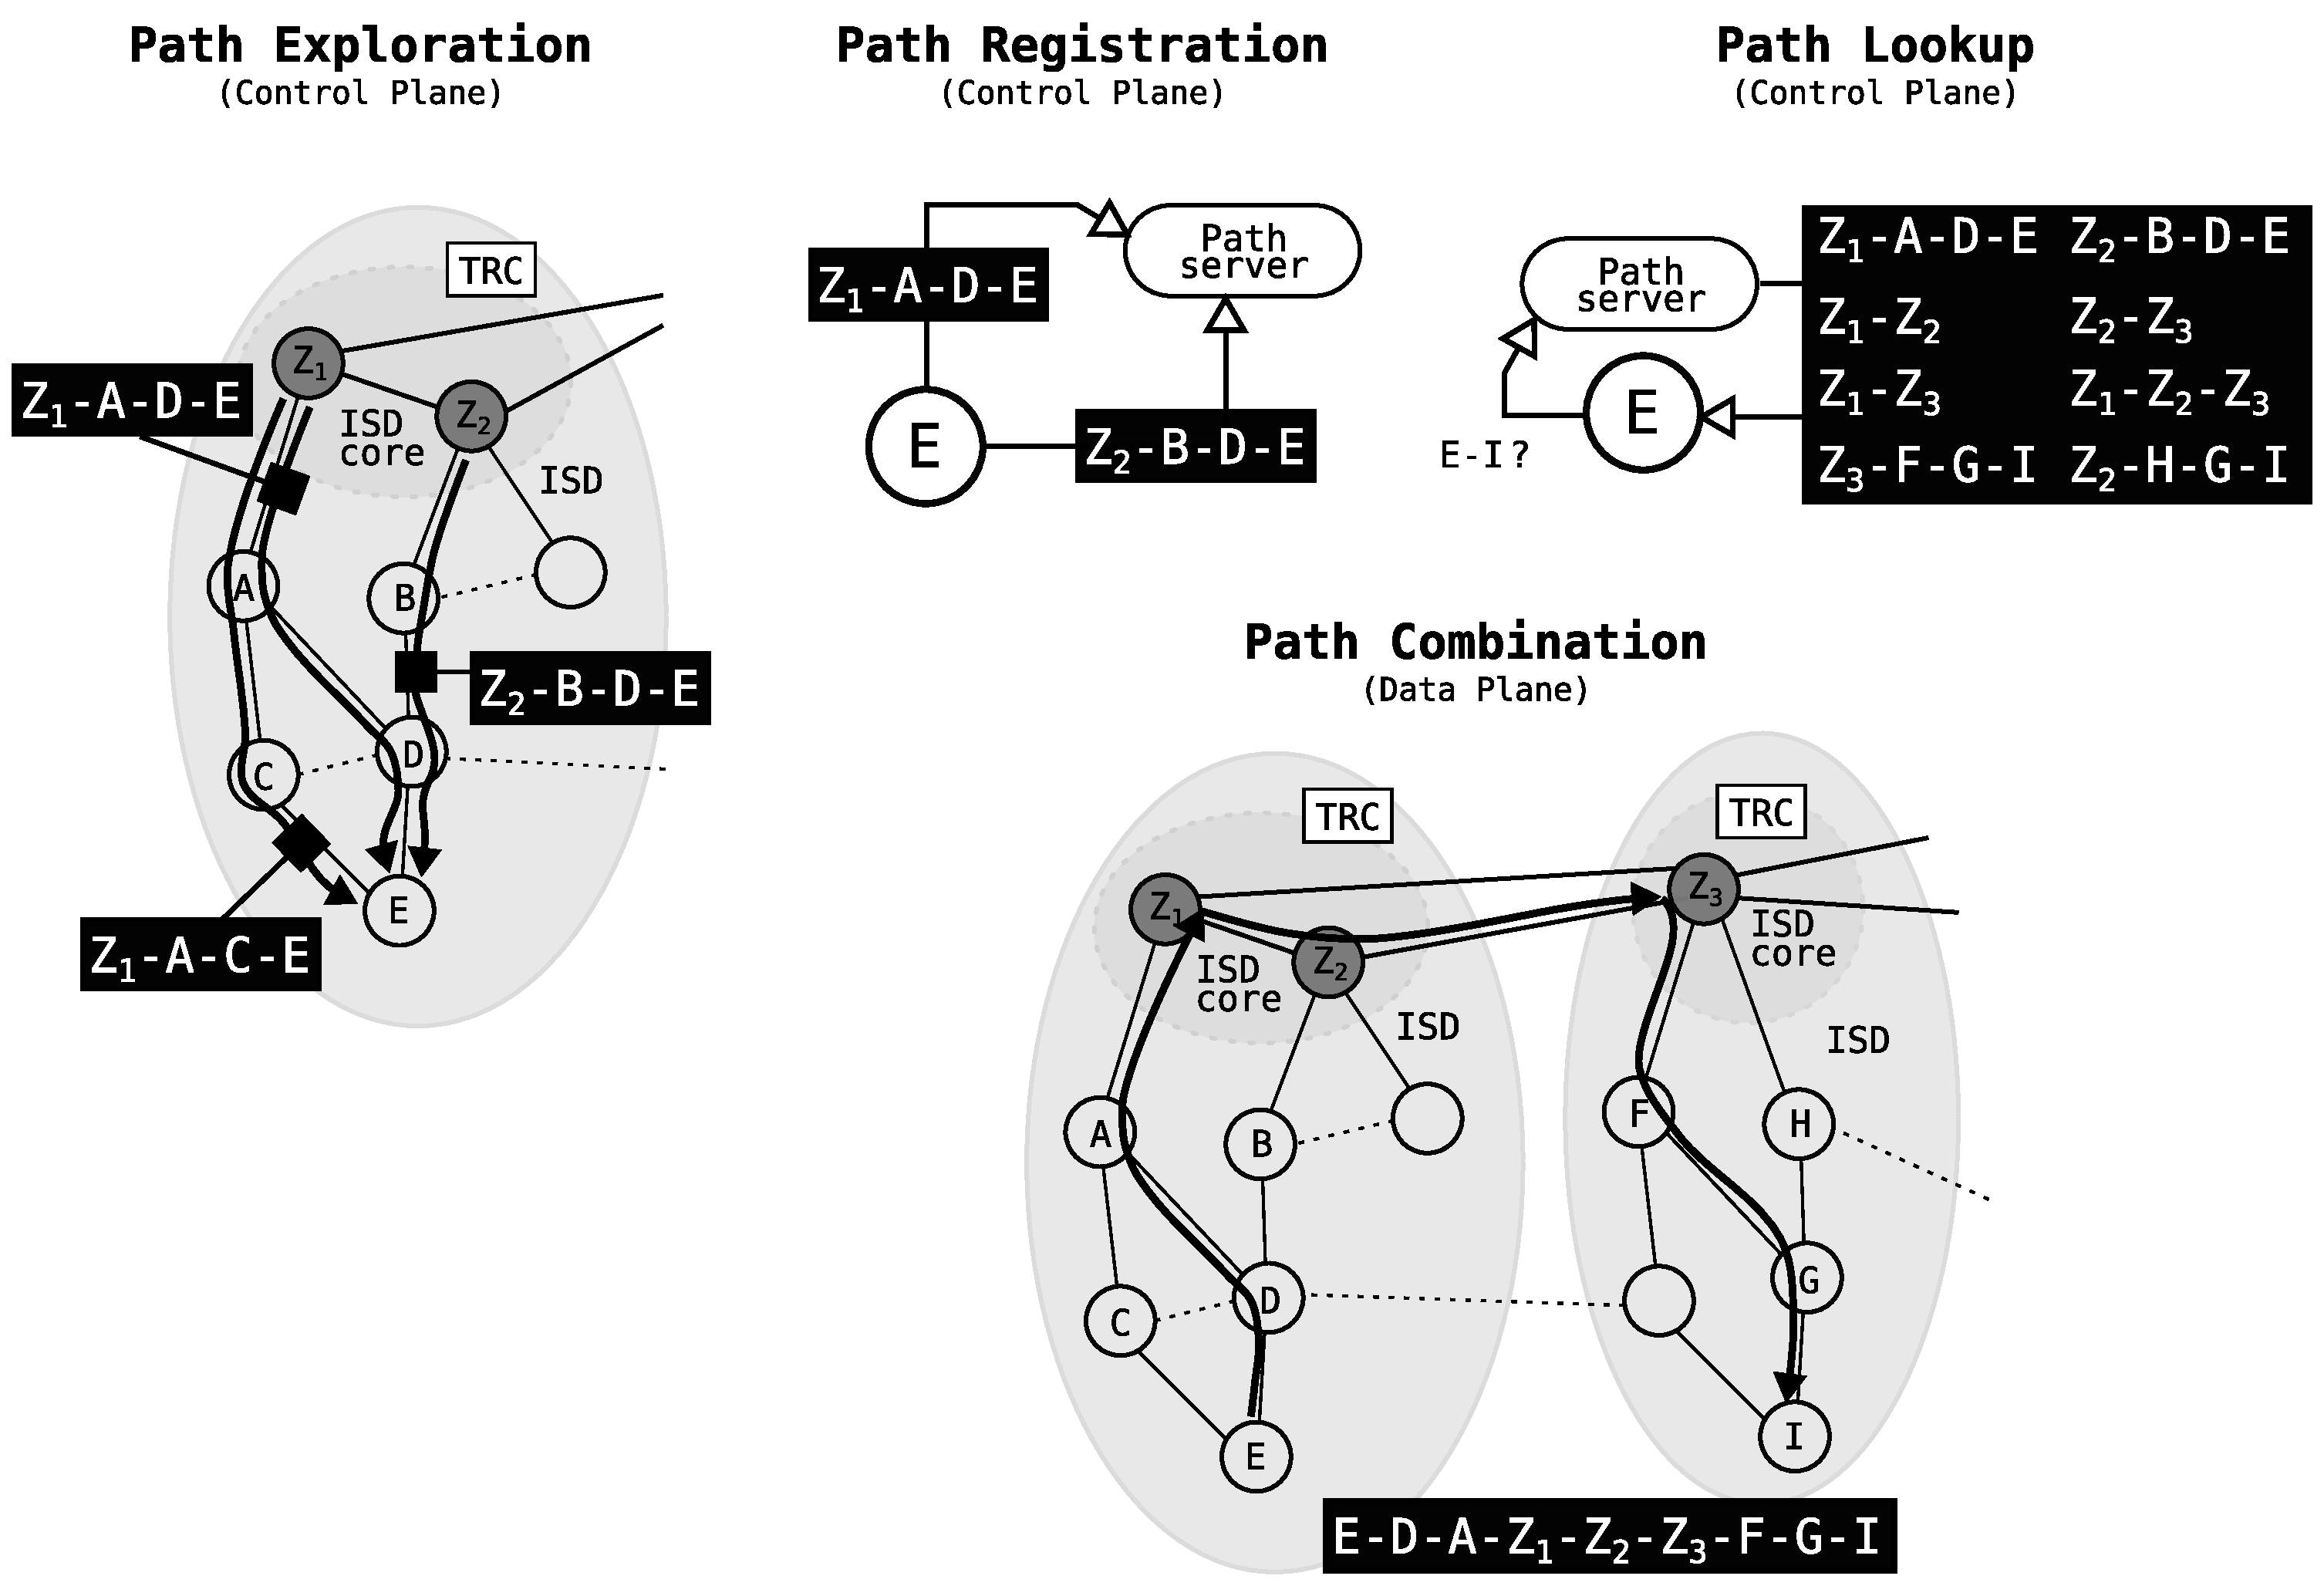
\includegraphics[scale=0.24]{../illustrations/importantConcepts/SCIONPathCreation.pdf} 
		\caption[]{Illustration of the different steps involved in the creation of a forwarding path: During path exploration, the AS E receives three PCB's describing different paths to reach the core. It decides to register two of these at the path server. If AS E wants to reach AS I it performs a lookup at the path server to get possible path segments. These individual path segments can then in the path combination be arbitrarily joined to form a forwarding path used for data exchange.}
		\label{fig:SCIONCreationForwardingPath}
	\end{center}
\end{figure}

\paragraph{Forwarding (Data Plane)}

Once a path is formed, it is included in the SCION packet header and used for forwarding. The recipient of a packet can send back data by simply inverting the path along where it got the packet or create a different one by performing a path lookup and combination on its own.

\subsection*{Conclusion}

This summary only scratches the surface of the functionality that SCION provides. The new internet architecture offers a variety of additional functions, security mechanisms and extensions which are not mentioned here. The goal of this section was to explain why the transformation to a new Internet architecture is so important and to introduce SCION as a promising candidate. Interested readers are again referred to the SCION book \cite{SCIONBook} or website \cite{SCIONWebMain}.